\chapter{Experimental Evaluation}
\label{chap:eval}

\section{Introduction}
\label{sec:eval-intro}

This chapter presents a comprehensive experimental evaluation of the I2C WASI interface implementations developed for WAMR and Wasmtime runtimes. It focuses on comparing their \textbf{performance characteristics} and \textbf{resource utilization}. The primary focus centers on a detailed comparative analysis between these two WebAssembly runtime approaches, while leveraging the native implementation as a performance baseline and reference point.

The evaluation encompasses \textbf{timing analysis} across multiple execution phases and comprehensive \textbf{memory profiling} to track allocation patterns. This data is then used for statistical analysis to ensure reliable and reproducible results. By systematically measuring runtime setup overhead, execution latency, and memory consumption, this experimental evaluation provides quantitative insights into the practical trade-offs between different WebAssembly runtime architectures.

This analysis directly addresses the second research question of this thesis: \textbf{RQ2: What is the performance impact of different WebAssembly runtime approaches?} Through controlled experimentation and statistical validation, the evaluation establishes an empirical foundation for understanding when and why specific runtime choices are optimal for embedded I2C applications.

\section{Evaluation Setup}
\label{sec:eval-methodology}

Having established the evaluation objectives and methodology in Section~\ref{sec:eval-intro}, this section details the used infrastructure for this analysis. The experimental setup encompasses three critical components: the hardware configuration that enables I2C communication, the firmware implementations of the I2C peripheral, and the software framework that facilitates accurate performance measurement and statistical analysis.

\subsection{Hardware Configuration}
\label{subsec:eval-setup-hw}

The experimental testbed consists of a Raspberry Pi acting as the I2C controller, connected to an Arduino Uno serving as the I2C peripheral \footnote{Modern naming conventions for I2C context prefer \textit{controller/peripheral} over \textit{master/slave}}.

\textbf{Controller Configuration:}
\begin{itemize}
    \item Board: \textit{Raspberry Pi 5}
    \item Architecture: \textit{ARM64} % TODO: reference pi datasheet
    \item Operating System: \textit{Raspberry Pi OS (Desktop features turned off)}
\end{itemize}

\textbf{Peripheral Configuration:}
\begin{itemize}
    \item Board: \textit{Arduino Uno R3 (ATmega328P)}
    \item Peripheral Address: \textit{0x09}
    \item Serial Interface: \textit{USB serial for correctness verification (disabled during performance tests)}
\end{itemize}

\begin{figure}[h]
	\centering
	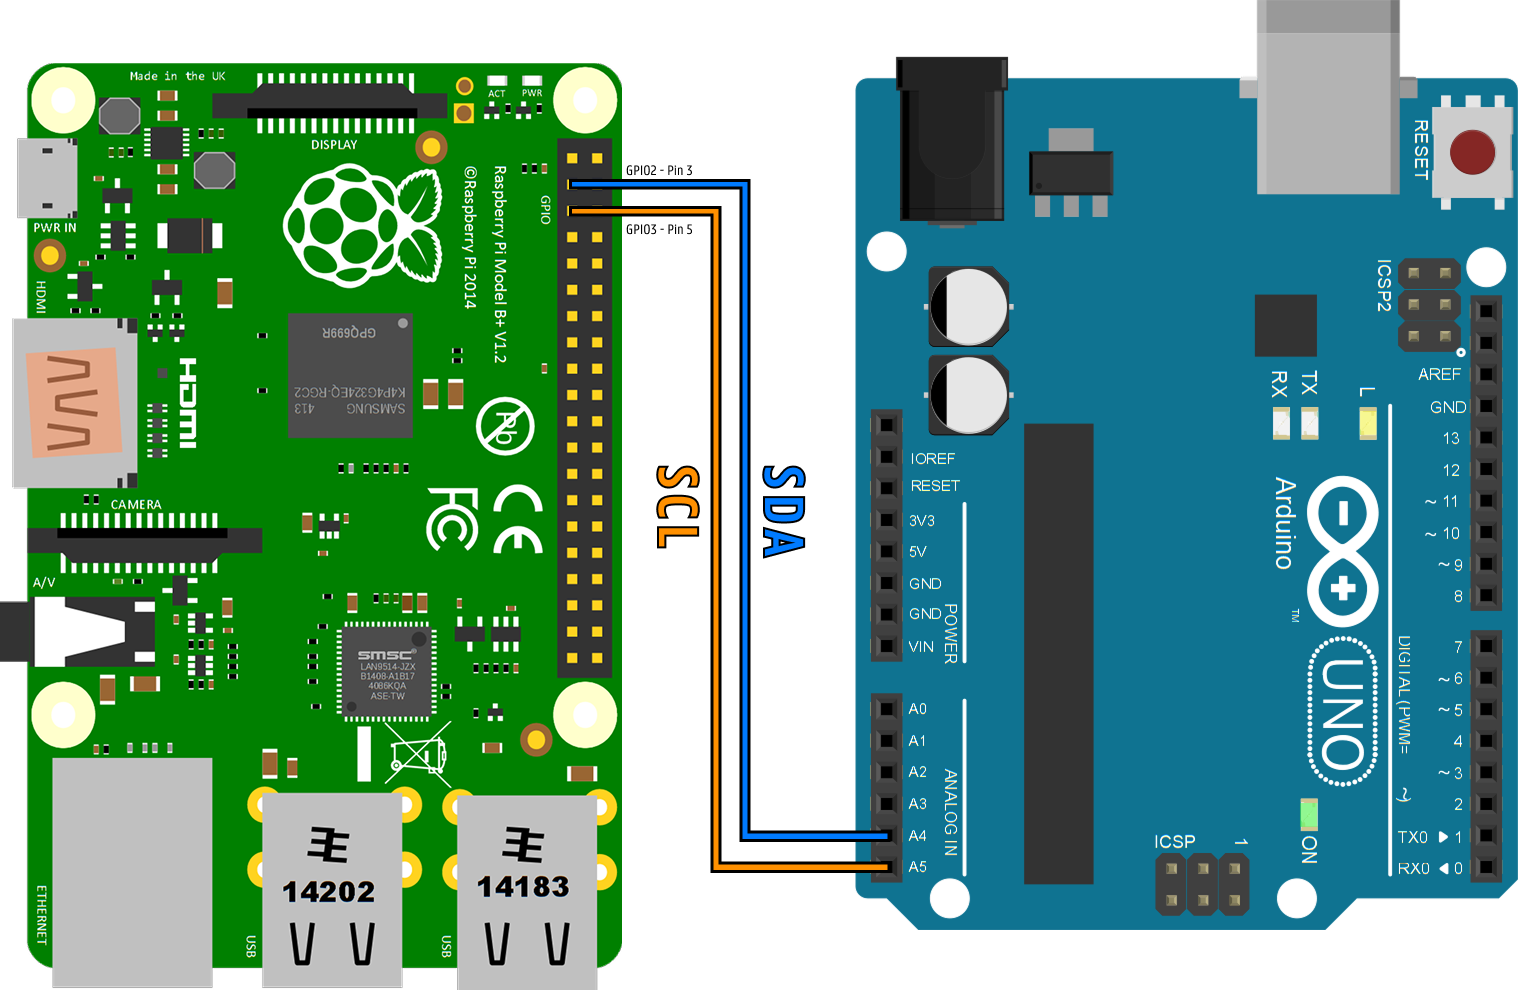
\includegraphics[width=0.7\textwidth]{images/HW_config.png}
	\caption{Hardware connection diagram.}
	\label{fig:hw-connection}
\end{figure}

\subsection{Arduino Firmware Implementation}
\label{subsec:eval-setup-fw}

Two firmware versions were developed for different evaluation phases:

\subsubsection{Correctness Verification Firmware}
This firmware implements echo functionality for debugging. All I2C transactions are logged via USB serial, enabling transaction verification.

\subsubsection{Performance Testing Firmware}
For performance benchmarks, an optimized firmware version was deployed that eliminates serial communication overhead. Upon receiving any I2C write request, the Arduino responds with a fixed ``hello'' message (\texttt{0x68, 0x65, 0x6c, 0x6c, 0x6f}) for one subsequent read operation. This approach minimizes Arduino-side processing variability and keeps extra overhead to a minimum.

\subsection{Benchmark Methodology}
\label{subsec:eval-setup-bench}

The evaluation follows a three-phase methodology to ensure correctness and robust measurement of latency and memory utilization.

\subsubsection{Phase 1: Correctness Verification}
Prior to performance measurement, functional correctness is verified by executing ping-pong operations across all implementations and confirming successful I2C transactions via Arduino serial monitor output.

\subsubsection{Phase 2: Performance Measurement}
Performance evaluation employs \textbf{Criterion.rs}, a statistical benchmarking framework that provides automatic outlier detection, distribution plotting, calculates achievable sample size prior to measurements during a warm-up phase and provides statistical insights post measurements\cite{criterion_rs}. The tool \texttt{cargo-criterion} provides machine-readable JSON output of those measurements, which allows us to also perform manual analysis and visualizations using Python/Jupyter.

The benchmark is divided into three different measurements, referred to as \textbf{Groups}. Each runtime gets evaluated over 100 samples according to the group's implementation:
\begin{itemize}
    \item \textbf{Runtime Setup:} Time to initialize runtime and prepare for I2C operations
    \item \textbf{Cold Execution:} A single ping-pong operation after a new runtime initialization
    \item \textbf{Hot Execution:} Repeated ping-pong operations in steady state
\end{itemize}

\subsubsection{Phase 3: Memory utilization}
% TODO: reference dhat
A single binary is built to run memory utilization profiling using DHAT. It initializes two profilers, measuring Runtime Setup and Guest execution.

\section{Runtime Setup Performance Analysis}
\label{sec:eval-setup}

Runtime initialization represents a critical performance dimension, particularly for embedded devices deployed in scenarios where Time-to-First-Execution is crucial. This section analyzes the setup overhead for each implementation and discusses the implications for practical deployment scenarios.

\subsection{Native Baseline}
\label{subsec:eval-setup-native}

The native implementation only using linux-embedded-hal provides the performance baseline for "runtime" initialization. Table~\ref{tab:native-setup} presents an overview of the measured characteristics, while Figure~\ref{fig:native-setup-distribution} gives a visual representation of the distribution.

\begin{table}[h]
    \centering
    \caption{Native Implementation's Setup overhead}
    \label{tab:native-setup}
    \begin{tabular}{cccc}
        \toprule
        \textbf{Mean (µs)} & \textbf{Median (µs)} & \textbf{Std Dev (ns)} & \textbf{95\% CI (µs)} \\
        \midrule
        1.9466 & 1.9483 & 10.5846 & [1.9445 ; 1.9487] \\
        \bottomrule
    \end{tabular}
\end{table}

\begin{figure}[h]
    \centering
    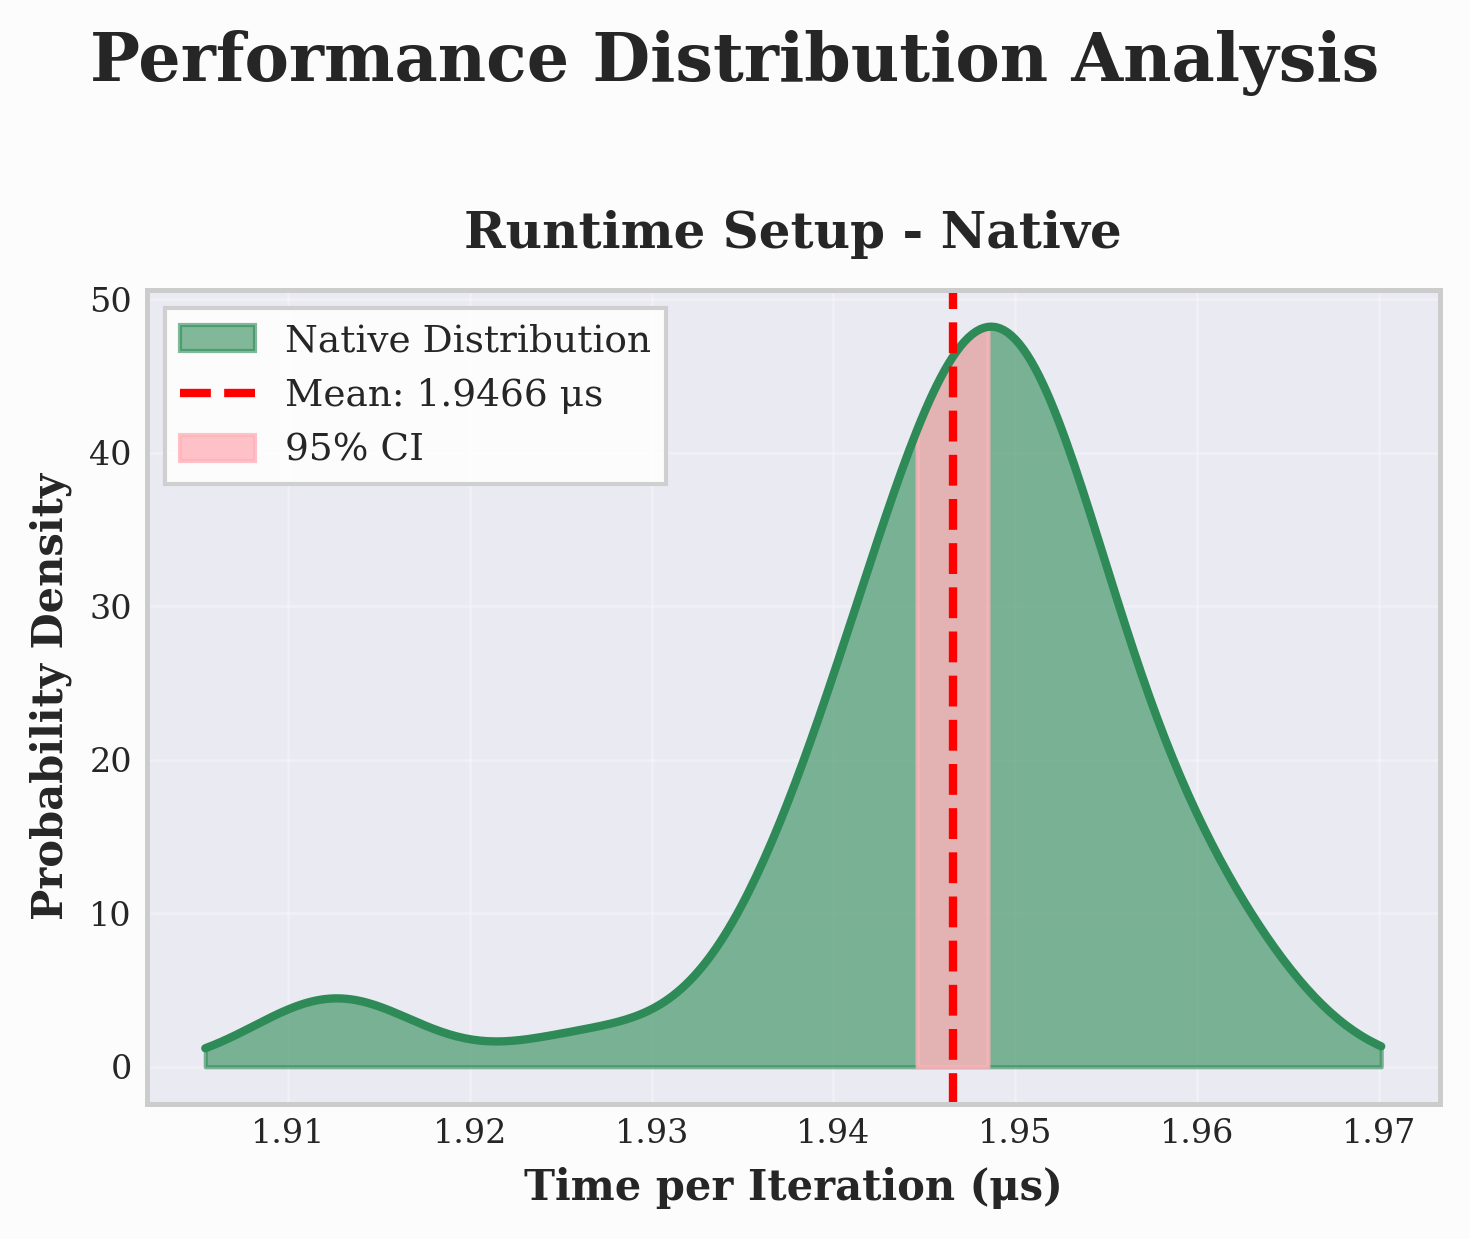
\includegraphics[width=0.7\textwidth]{images/native-setup-distribution}
    \caption{Distribution of Native Runtime Setup measurements}
    \label{fig:native-setup-distribution}
\end{figure}

While the native implementation is categorized under Runtime Setup, it does not involve any runtime initialization. Instead, it establishes a performance baseline by measuring the Linux I2C Stack overhead for opening the \texttt{/dev/i2c-1} device file. Since the \acrshort{wasm} implementations utilize the same underlying Linux I2C software stack, this baseline enables quantification of the additional overhead introduced purely by runtime instantiation when compared against the \acrshort{wasm} implementations.

\subsection{WebAssembly Comparison}
\label{subsec:eval-setup-wasm}

Table~\ref{tab:wasm-setup} presents the initialization overhead for \acrshort{wamr} and Wasmtime implementations. Figure~\ref{fig:wasm-setup-distribution} gives a visual representation.

\begin{table}[h]
    \centering
    \caption{\acrshort{wasm} Implementations's Runtime Setup overhead comparison}
    \label{tab:wasm-setup}
    \begin{tabular}{lcccc}
        \toprule
        \textbf{Implementation} & \textbf{Mean (µs)} & \textbf{Median (µs)} & \textbf{Std Dev (ns)} & \textbf{95\% CI (µs)} \\
        \midrule
        WAMR        & 253.1126 & 253.1301 & 258.4145 & [253.0613 ; 253.1638] \\
        Wasmtime    & 19,559.1592 & 19,559.8473 & 11,656.5225 & [19,556.8463 ; 19,561.4721] \\
        \bottomrule
    \end{tabular}
\end{table}

\begin{figure}[h]
    \centering
    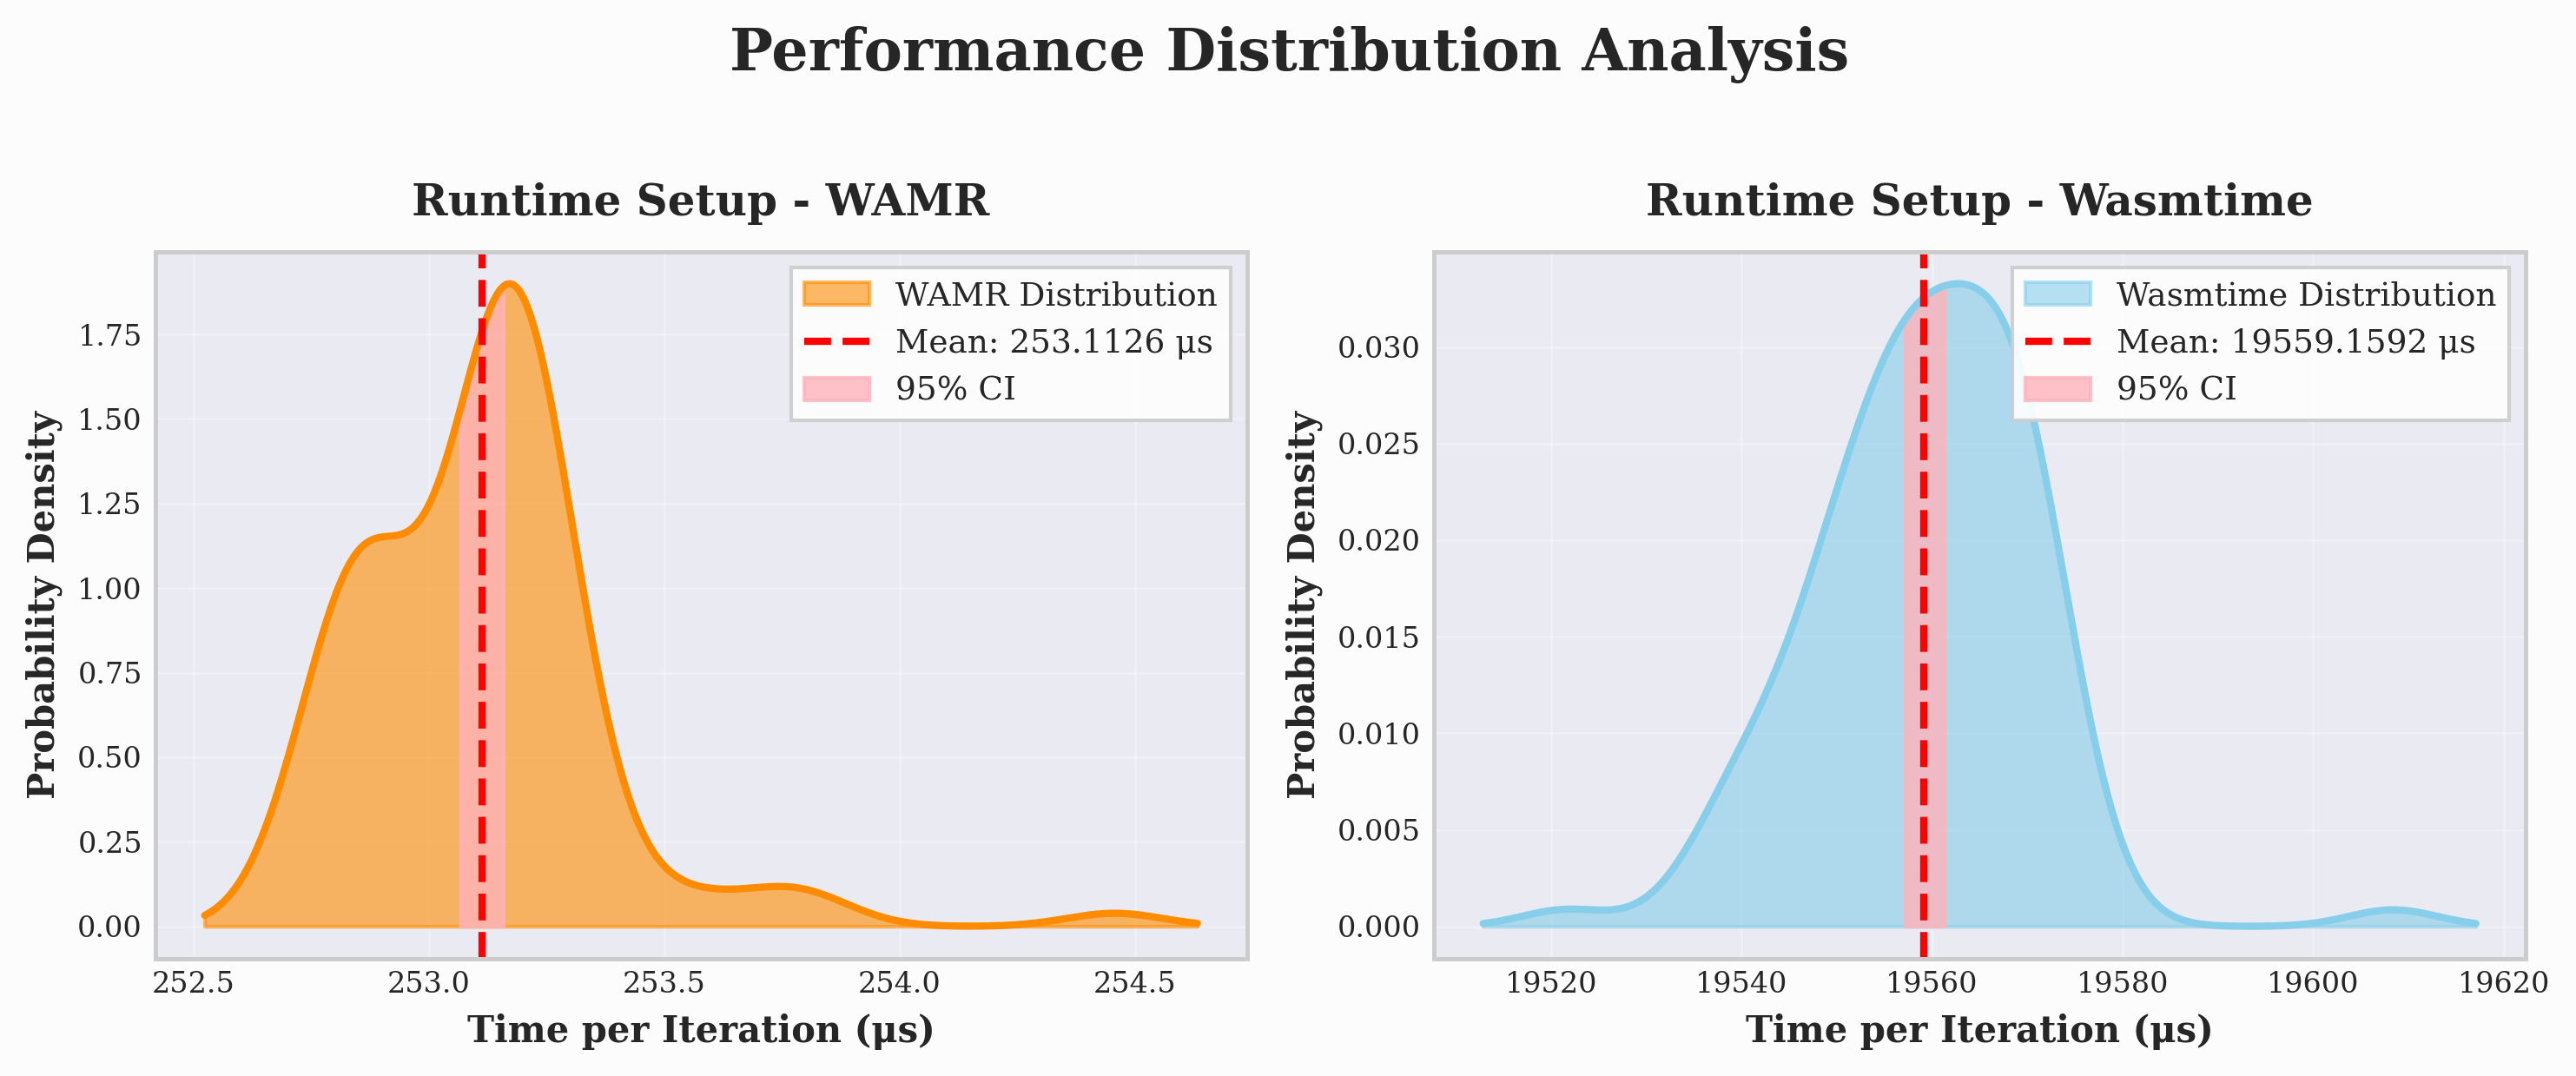
\includegraphics[width=0.9\textwidth]{images/wasm-setup-distribution}
    \caption{Distributions of \acrshort{wasm} Runtime Setup measurements}
    \label{fig:wasm-setup-distribution}
\end{figure}

\subsubsection{Setup Performance Analysis}
The results reveal a dramatic performance disparity between the two WebAssembly runtimes. \acrshort{wamr} achieves setup initialization in approximately 253 μs, representing 130x overhead compared to the native implementation. However, Wasmtime exhibits substantially higher initialization costs at 19.6 ms, creating just over 10,000x overhead relative to native and 77x overhead compared to \acrshort{wamr}. Figure~\ref{fig:wasm-setup-relative} gives an overview.

\begin{figure}[h]
    \centering
    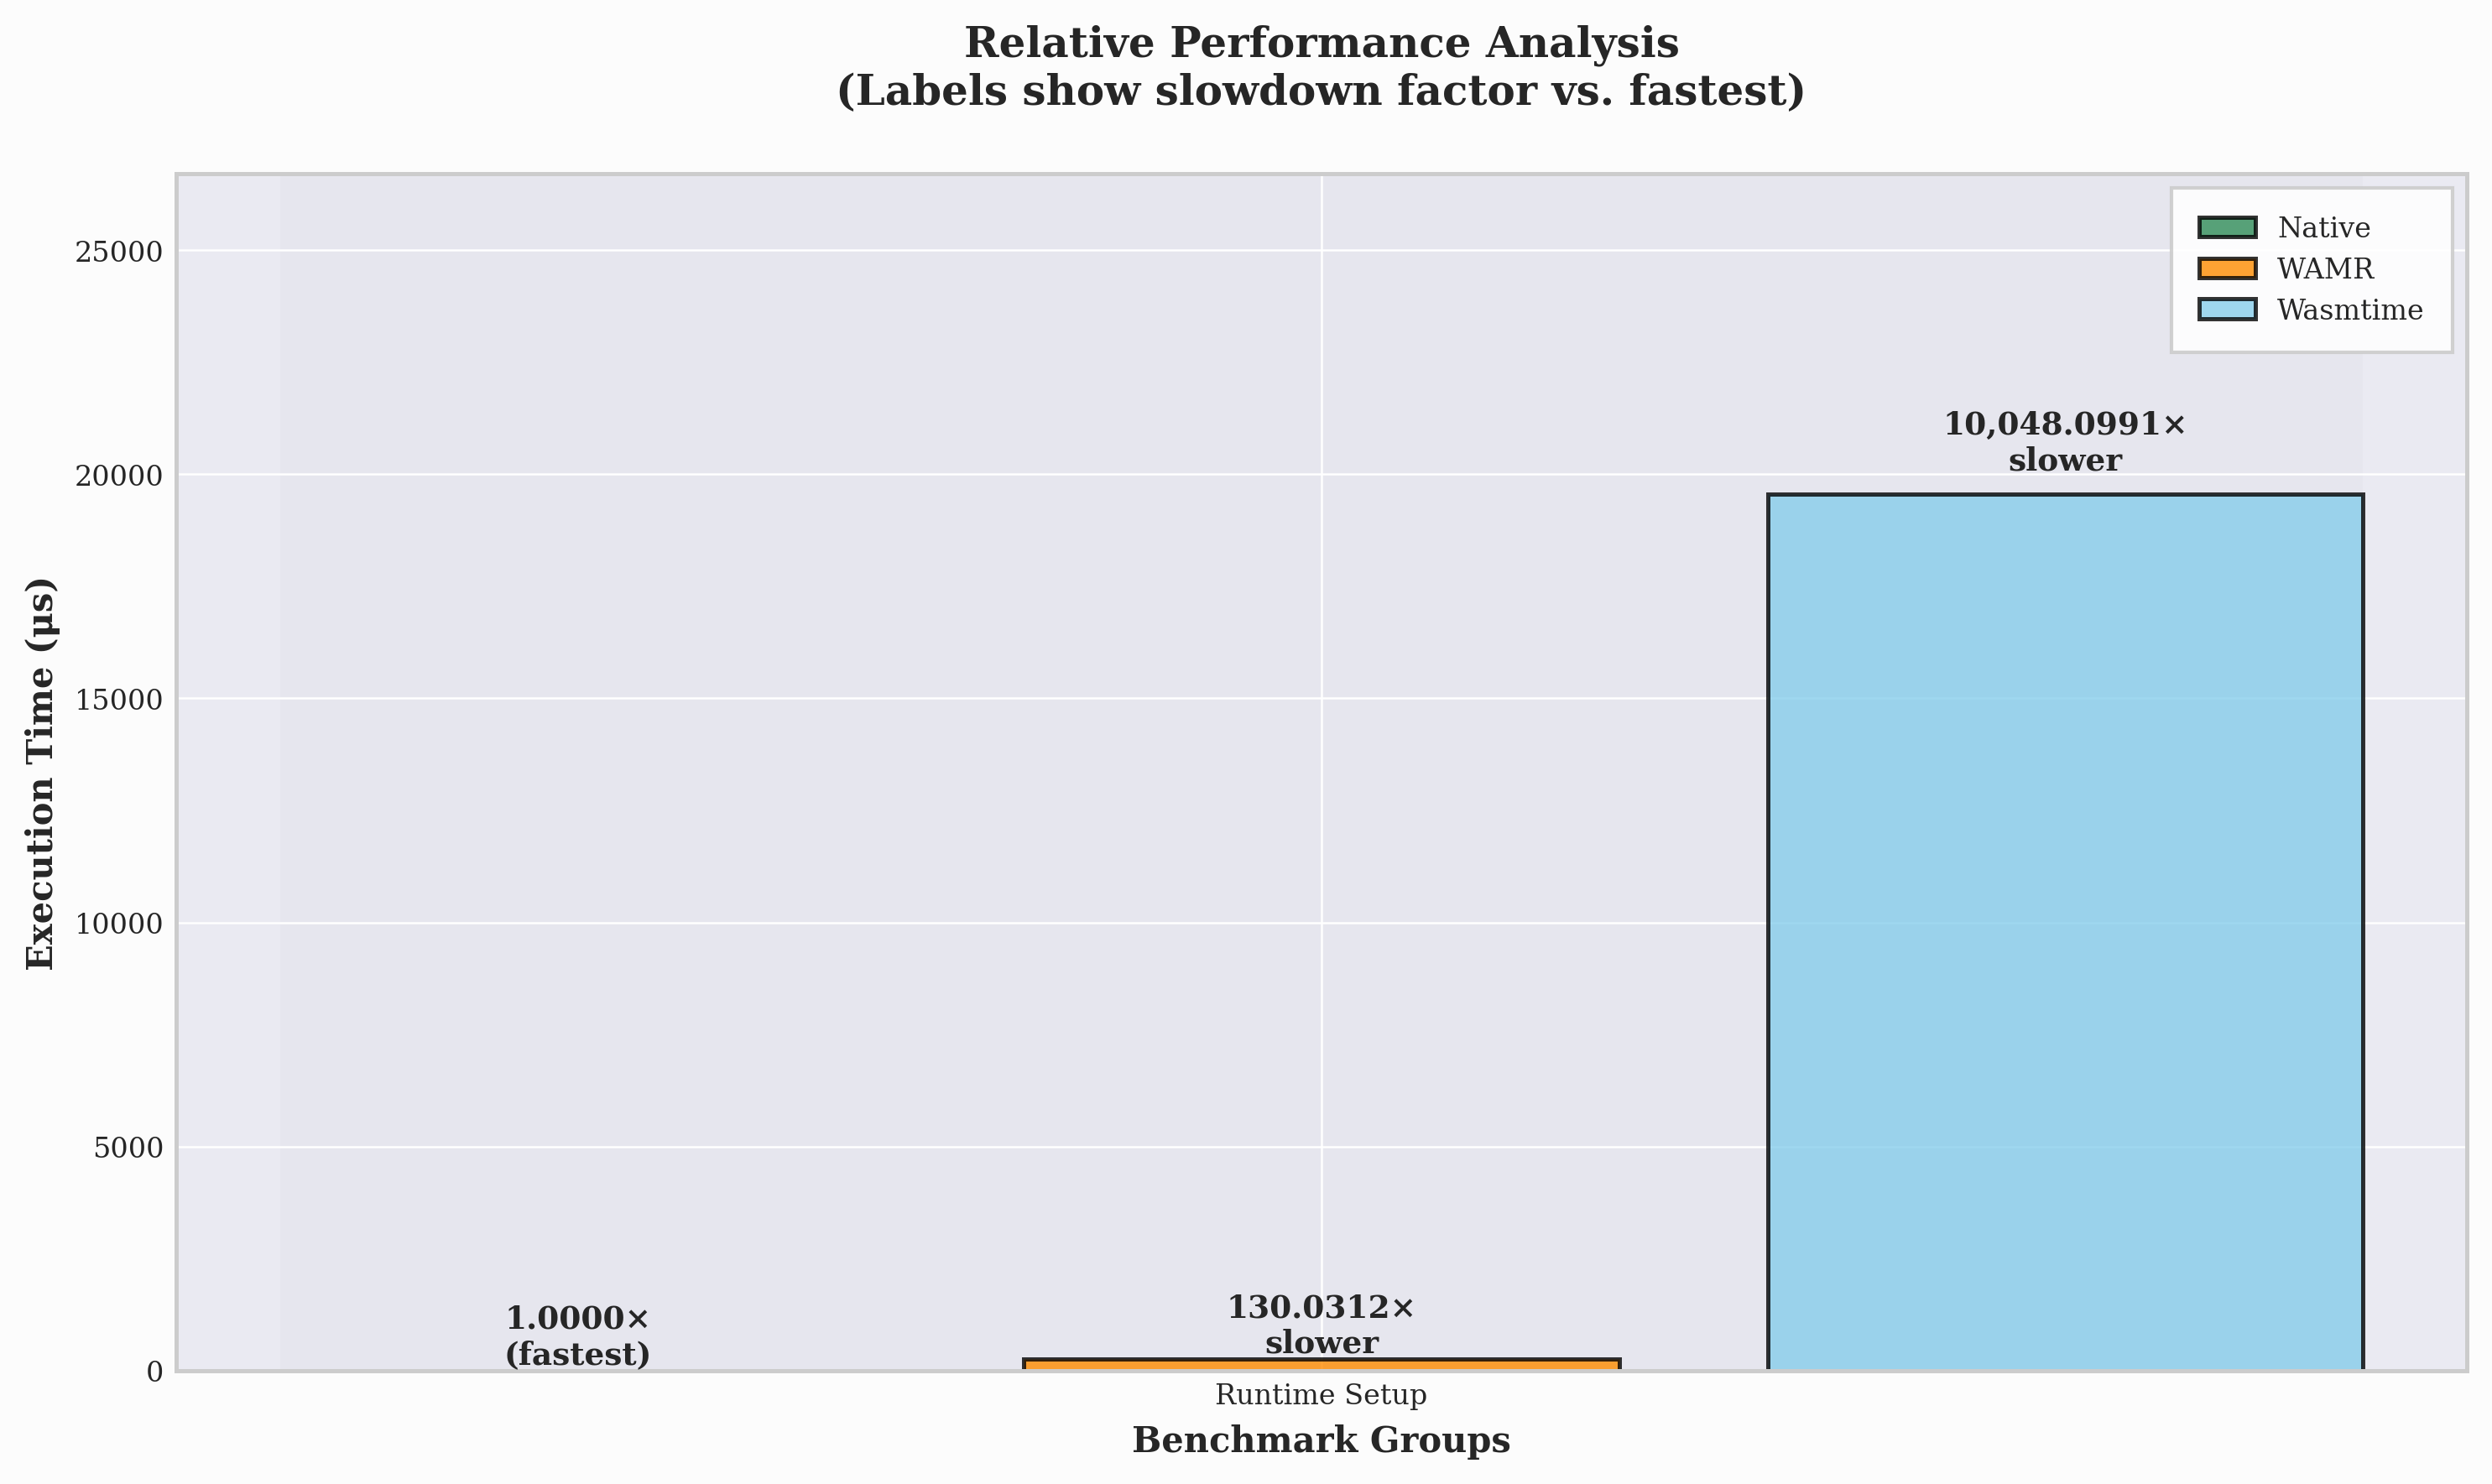
\includegraphics[width=0.9\textwidth]{images/wasm-setup-relative}
    \caption{Comparison of \acrshort{wasm} Implementation's Runtime Setup relative to the baseline}
    \label{fig:wasm-setup-relative}
\end{figure}

\subsection{Embedded Application Implications}
\label{subsec:setup-implications}

These setup time characteristics have profound implications for embedded deployment patterns. For example:

\textbf{Ultra Low Power devices:} Scenarios where Ultra Low Power devices are completely turned off, making them lose their state. Having to instantiate a new Wasmtime runtime would take up too much power. Even \acrshort{wamr} could bring too much overhead, but when virtualization advantages are required, \acrshort{wasm} features could make \acrshort{wamr} viable.

\textbf{Real-time Systems:} Applications requiring deterministic startup behavior within millisecond constraints would exclude Wasmtime entirely, while \acrshort{wamr}'s sub-millisecond setup remains viable for many real-time scenarios.

\textbf{Long-running Applications:} Conversely, applications with infrequent instantiation (e.g., edge computing services) can amortize Wasmtime's setup cost over extended execution periods.

\section{Execution Performance Analysis}
\label{sec:eval-execution}

With runtime initialization complete, this section examines the steady-state execution performance for I2C operations, comparing cold (first-execution) and hot (repeated-execution) characteristics.

\subsection{Native Baseline}
\label{subsec:eval-execution-native}

Table~\ref{tab:native-execution} establishes the native performance baseline for I2C ping-pong operations.

\begin{table}[h]
    \centering
    \caption{Native Implementation Execution Performance}
    \label{tab:native-execution}
    \begin{tabular}{lcccc}
        \toprule
        \textbf{Execution Type} & \textbf{Mean (µs)} & \textbf{Median (µs)} & \textbf{Std Dev (ns)} & \textbf{95\% CI (µs)} \\
        \midrule
        Cold Execution  & 594.5275 & 594.5636 & 281.8579 & [594.4715 ; 594.5834] \\
        Hot Execution   & 589.0368 & 589.0307 & 69.9196 & [589.0230 ; 589.0507] \\
    \end{tabular}
\end{table}

\subsection{WebAssembly Comparison}
\label{subsec:eval-execution-wasm}

Tables \ref{tab:wasm-execution-cold} and \ref{tab:wasm-execution-hot} compare execution performance between WAMR and Wasmtime for both cold and hot execution scenarios respectively.

\begin{table}[h]
    \centering
    \caption{WebAssembly Cold Execution Performance Comparison}
    \label{tab:wasm-execution-cold}
    \begin{tabular}{lcccc}
        \toprule
        \textbf{Implementation} & \textbf{Mean (µs)} & \textbf{Median (µs)} & \textbf{Std Dev (ns)} & \textbf{95\% CI (µs)} \\
        \midrule
        WAMR      & 1,211.0415 & 1,210.9849 & 5,144.4222 & [1,210.0207 ; 1,212.0622] \\
        Wasmtime  & 1,301.8975 & 1,300.5868 & 4,895.5251 & [1,300.9262 ; 1,302.8689] \\
        \bottomrule
    \end{tabular}
\end{table}

\begin{table}[h]
    \centering
    \caption{WebAssembly Hot Execution Performance Comparison}
    \label{tab:wasm-execution-hot}
    \begin{tabular}{lcccc}
        \toprule
        \textbf{Implementation} & \textbf{Mean (µs)} & \textbf{Median (µs)} & \textbf{Std Dev (ns)} & \textbf{95\% CI (µs)} \\
        \midrule
        WAMR      & 1,185.4778 & 1,185.8310 & 673.0608 & [1,185.3442 ; 1,185.6113] \\
        Wasmtime  & 1,184.4430 & 1,184.2941 & 522.5048 & [1,184.3393 ; 1,184.5467] \\
        \bottomrule
    \end{tabular}
\end{table}

\subsubsection{Key Execution Performance Findings:}

\begin{figure}[h]
    \centering
    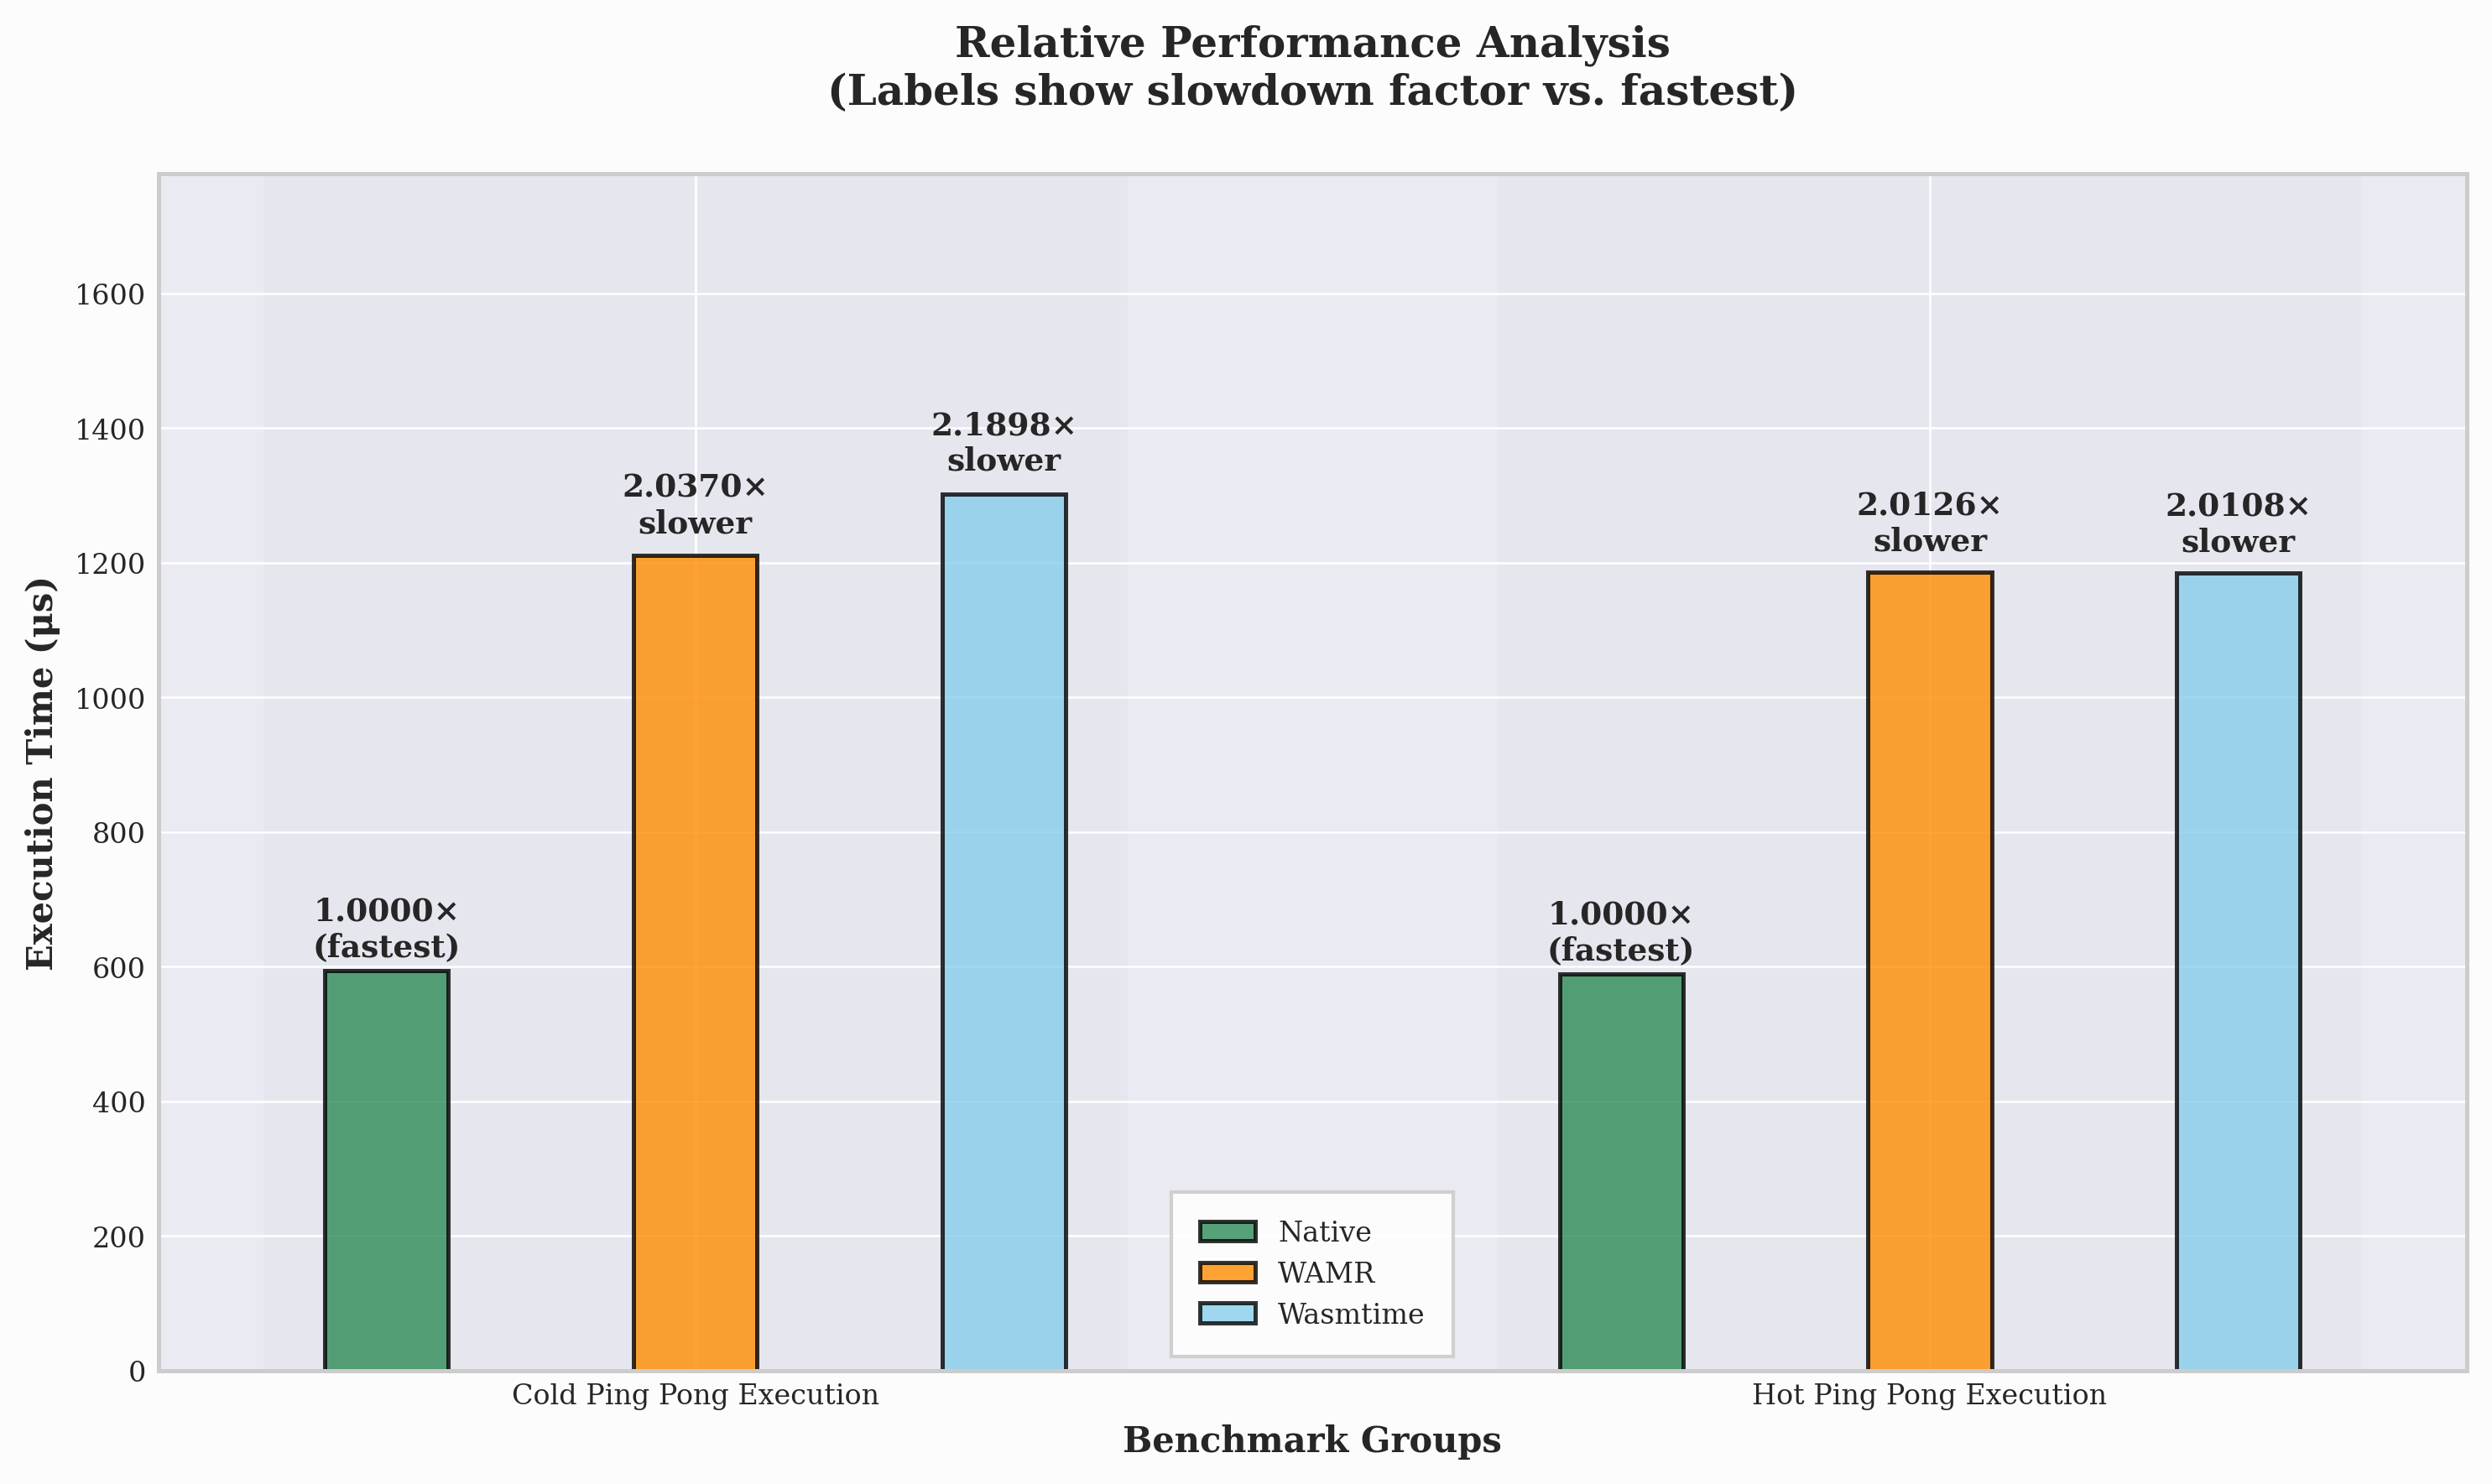
\includegraphics[width=1.0\textwidth]{images/wasm-execution-relative}
    \caption{Execution Performance Comparison: Native vs \acrshort{wamr} vs Wasmtime}
    \label{fig:wasm-execution-relative}
\end{figure}

\begin{enumerate}
    \item \textbf{Convergent Steady-State Performance:} Both WAMR and Wasmtime achieve remarkably similar hot execution performance 2x native overhead, despite their architectural differences.

    \item \textbf{Statistical difference:} Although the Cold Execution would statistically be considered significantly different, a practical difference of only 90 µs is considered negligible.
    
    \item \textbf{Minimal Cold/Hot Differences:} Minimal cold/hot differences for WAMR (2.1\% improvement), with Wasmtime showing moderate optimization benefits (9.0\% improvement), suggesting some caching or optimization effects.
    
    \item \textbf{Consistent WebAssembly Overhead:} Both implementations exhibit approximately 2x overhead compared to native execution, representing the cost of WebAssembly instruction execution and host function call marshalling.
\end{enumerate}

\subsection{Performance Variability Assessment}
\label{subsec:eval-execution-variability}

Table~\ref{tab:variability} presents Coefficient of Variation (CV) metrics to assess performance consistency across implementations. Figure~\ref{fig:variability-comparison}

\begin{table}[h]
    \centering
    \caption{Performance Variability Comparison (Coefficient of Variation)}
    \label{tab:variability}
    \begin{tabular}{lccc}
    \toprule
    \textbf{Implementation} & \textbf{Setup CV (\%)} & \textbf{Cold Exec CV (\%)} & \textbf{Hot Exec CV (\%)} \\
    \midrule
    Native       & 0.5438 & 0.0474 & 0.0119 \\
    WAMR         & 0.1021 & 0.4248 & 0.0568 \\
    Wasmtime     & 0.0596 & 0.3760 & 0.0441 \\
    \bottomrule
    \end{tabular}
\end{table}

\begin{figure}[h]
    \centering
    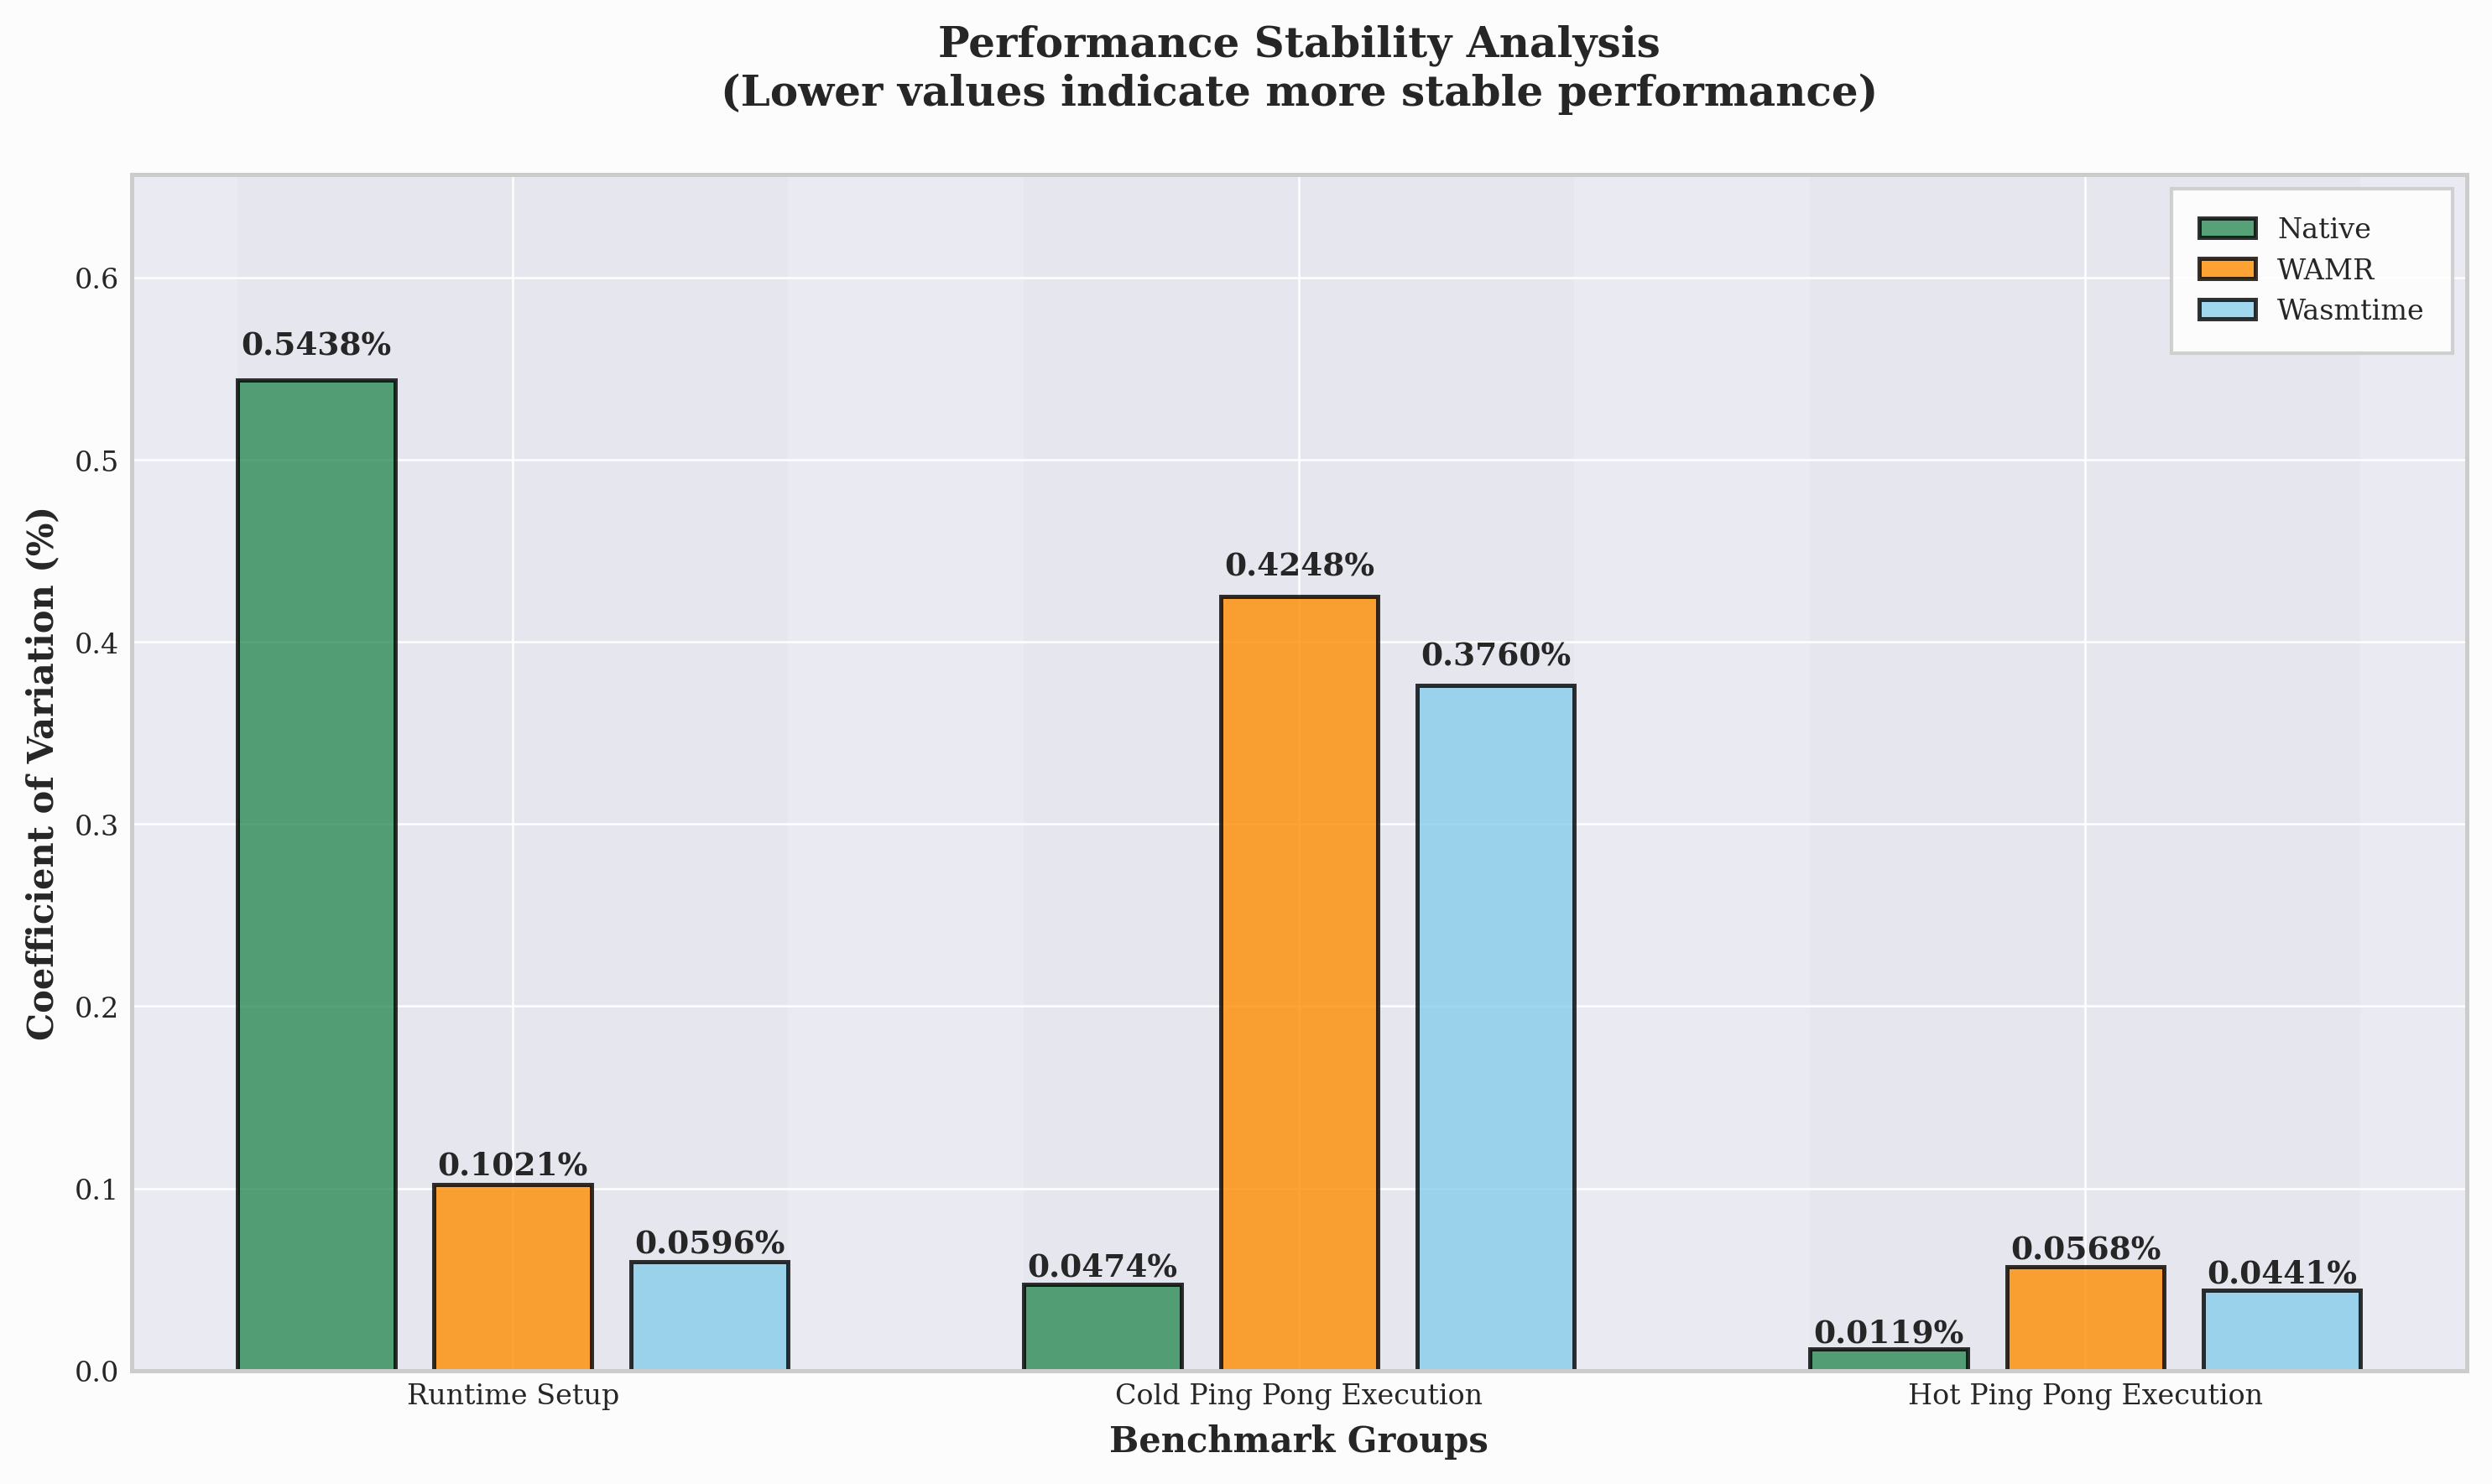
\includegraphics[width=0.9\textwidth]{images/variability-comparison}
    \caption{Comparison of calculated Coefficient of Variation across all implementations}
    \label{fig:variability-comparison}
\end{figure}

The performance variability analysis reveals distinct consistency patterns across the three implementations. During the setup phase, the native implementation exhibits the highest variability (0.54\% CV), suggesting that direct hardware initialization is less predictable or stable, while Wasmtime demonstrates the most consistent setup behavior (0.06\% CV). This pattern reverses during cold execution, where both WebAssembly runtimes show significantly higher variability (WAMR: 0.42\%, Wasmtime: 0.38\%) compared to the native implementation (0.047\%). This increased variability can be attributed to the complex initialization and optimization processes within the WebAssembly runtimes during first execution. However, during hot execution, all implementations converge to low variability levels, with the native implementation achieving the highest consistency (0.012\% CV), followed by Wasmtime (0.044\%) and WAMR (0.057\%). Importantly, all Coefficient of Variation values remain well below 1\%, indicating that despite relative differences between implementations, all approaches demonstrate excellent measurement consistency and predictable performance characteristics.

\section{Memory Usage Analysis}
\label{sec:eval-memory}

Memory consumption patterns provide critical insights for embedded applications with constrained resources. This section analyzes heap allocation behavior during both runtime setup and execution phases using DHAT profiling.

\subsection{Runtime Setup Memory Profiling}
\label{subsec:memory-setup}

Table~\ref{tab:memory-setup} presents memory allocation characteristics during runtime initialization, revealing the resource requirements for each implementation approach.

\begin{table}[h]
    \centering
    \caption{Memory Usage During Runtime Setup}
    \label{tab:memory-setup}
    \begin{tabular}{lccc}
        \toprule
        \textbf{Implementation} & \textbf{Total (bytes)} & \textbf{Peak (bytes)} & \textbf{Blocks (count)} \\
        \midrule
        Native        & 10          & 10        & 1 \\
        WAMR          & 10,124      & 10,080    & 16 \\
        Wasmtime      & 14,247,171  & 2,716,728 & 16,686 \\
        \bottomrule
    \end{tabular}
\end{table}

\subsubsection{Setup Memory Analysis}

The memory allocation patterns during runtime initialization reveal fundamental architectural differences between the implementations. The native implementation establishes a minimal baseline with just 10 bytes allocated, reflecting direct hardware access without abstraction overhead.

WAMR demonstrates embedded-friendly resource consumption, requiring approximately 10KB across 16 allocation blocks. This three-order-of-magnitude increase over native remains acceptable for most embedded systems, particularly given that 99.6\% of allocated memory persists throughout the runtime lifecycle—indicating efficient, stable memory management without excessive allocation churn.

Wasmtime's memory profile reflects its sophisticated execution engine architecture. While total allocations reach 14.2MB during initialization, the runtime maintains only 2.7MB at peak usage. This 81\% temporary allocation ratio reveals intensive memory operations during JIT compilation and module optimization. The 16,686 allocation blocks (over 1,000x more than WAMR) further illustrate the complexity of component model instantiation and type system initialization.

These patterns directly impact deployment feasibility: WAMR's 10KB footprint fits comfortably within typical embedded constraints (even sub-MB microcontrollers), while Wasmtime's multi-megabyte requirements restrict it to more capable embedded Linux platforms. The correlation between memory complexity and setup time (77x difference) suggests that memory allocation overhead contributes significantly to initialization latency.

% TODO: decide on OLD or new content
% \subsubsection{Setup Memory Analysis:}
% The memory consumption analysis during runtime setup reveals dramatic differences in resource requirements across implementations, with implications spanning several orders of magnitude. The \textbf{native }implementation demonstrates minimal memory overhead, allocating only 10 bytes in a single allocation block, reflecting the direct hardware access approach with virtually no abstraction layer overhead. This establishes an extremely lean baseline that showcases the efficiency of direct I2C library usage.

% \textbf{WAMR} presents a moderate memory footprint, consuming 10,124 bytes (approximately 10KB) total allocation with a peak usage of 10,080 bytes across 16 allocation blocks. This represents a three-order-of-magnitude increase compared to the native implementation, yet remains within reasonable bounds for embedded applications. The close alignment between total and peak memory usage (10,124 vs 10,080 bytes) demonstrates that WAMR maintains most allocated memory throughout the setup process, indicating a relatively stable memory profile with minimal temporary allocations.

% In stark contrast, \textbf{Wasmtime} exhibits substantially higher memory requirements, allocating 14,247,171 bytes (approximately 14.2 MB) total across 16,686 allocation blocks during setup. However, the peak memory usage of 2,716,728 bytes (approximately 2.7 MB) reveals that roughly 81\% (\(\frac{Total-Peak}{Total}\)) of allocated memory consists of temporary allocations that are freed during the setup process. This pattern indicates intensive memory churning during runtime initialization, likely associated with JIT compilation, module loading, and optimization processes inherent to Wasmtime's sophisticated execution engine.

% The allocation \textbf{block count provides additional insight} into memory management patterns. While the native implementation requires only a single allocation, WAMR uses 16 blocks, suggesting modular memory organization. Wasmtime's 16,686 allocation blocks demonstrate the complex memory management required for its advanced runtime features, including component model support and aggressive optimization strategies.

% From an \textbf{embedded systems perspective}, these results highlight critical deployment considerations. WAMR's 10 KB memory overhead remains feasible for many embedded applications, while Wasmtime's multi-megabyte requirements may exceed available memory in resource-constrained environments. The memory consumption patterns also correlate with the observed setup performance differences, where Wasmtime's extensive memory allocation activity contributes to its longer initialization times, while WAMR's moderate memory footprint aligns with its faster setup performance.

\subsubsection{Execution Memory Efficiency}

Post-initialization memory requirements reveal excellent steady-state efficiency for both WebAssembly runtimes. These measurements capture only the incremental allocations required for guest function execution, independent of the established runtime footprint.

Both runtimes demonstrate remarkable efficiency: WAMR requires 327 bytes across 6 allocations, while Wasmtime uses 416 bytes across 10 allocations—a negligible 89-byte difference despite their architectural disparities. Compared to the 16-byte native baseline, this represents approximately 20-26x overhead, primarily attributable to WASI interface marshalling and guest-host communication buffers.

The minimal peak-to-total allocation differences (WAMR: 5\%, Wasmtime: 17\%) indicate stable execution without memory leaks or excessive temporary allocations. This efficiency validates both runtimes for long-running embedded applications where thousands of I2C operations must execute within constrained memory budgets.

Critically, these results demonstrate that the substantial initialization costs—particularly Wasmtime's 14.2MB—do not translate to proportional execution overhead. Once initialized, both runtimes operate within hundreds of bytes, making the initialization cost a one-time investment that can be amortized across the application lifetime.

\begin{table}[htbp]
    \centering
    \caption{Memory Usage During Ping-Pong Execution}
    \label{tab:memory-execution}
    \begin{tabular}{lrrr}
        \toprule
        \textbf{Implementation} & \textbf{Total (bytes)} & \textbf{Peak (bytes)} & \textbf{Blocks (count)} \\
        \midrule
        Native        & 16   & 16  & 1 \\
        WAMR          & 327  & 311 & 6 \\
        Wasmtime      & 416  & 347 & 10 \\
        \bottomrule
    \end{tabular}
\end{table}

% TODO: Decide on OLD or new content
% \subsection{Execution Memory Profiling}
% \label{subsec:memory-execution}

% Table~\ref{tab:memory-execution} analyzes memory allocation patterns during ping-pong execution, focusing on runtime overhead and potential memory leaks.



% \subsubsection{Execution Memory Efficiency:}
% The memory consumption during ping-pong execution reveals the incremental memory overhead required for actual I2C operation execution, measured independently from the established runtime footprint. Since these measurements capture only the additional allocations occurring during guest function execution (after runtime initialization is complete), they provide insight into the operational memory efficiency of each approach.

% The \textbf{native} implementation requires 16 bytes in a single allocation block specifically for executing the ping-pong I2C operation. This represents the pure memory cost of the I2C transaction, including data buffers and operation state management without any runtime abstraction overhead.

% \textbf{WAMR} demonstrates remarkably efficient execution memory usage, requiring only 327 bytes total with a peak usage of 311 bytes across 6 allocation blocks. This modest overhead represents the additional memory needed by the WebAssembly runtime to execute the guest function, manage the WASI I2C interface calls, and handle parameter marshaling between the WebAssembly module and the host I2C implementation. The minimal difference between total and peak allocations (16 bytes, approximately 4.9\%) indicates that WAMR maintains very stable memory usage during execution with virtually no temporary allocation churn.

% \textbf{Wasmtime} requires 416 bytes total allocation with a peak usage of 347 bytes distributed across 10 allocation blocks for execution. While this represents the highest overhead among the implementations, the absolute increment remains modest at approximately 26 times the native requirement and only 1.27 times the WAMR requirement. The 69 bytes difference between total and peak usage (16.6\%) suggests slightly more dynamic memory management during execution, potentially related to component model overhead.

% These results are particularly significant because they demonstrate that \textbf{both WebAssembly runtimes achieve very efficient steady-state execution}. After absorbing the substantial initialization costs (especially Wasmtime's 14.2MB setup overhead), the incremental memory required for actual I2C operations remains in the hundreds of bytes range. This profile makes both runtimes highly suitable for embedded applications performing repeated I2C operations, where the setup cost can be amortized and the per-operation overhead remains minimal.


\section{Discussion and Implications}
\label{sec:eval-discussion}

\subsection{Key Findings Summary}
\label{subsec:eval-discussion-keyfindings}

The experimental evaluation reveals critical insights addressing the WebAssembly runtime performance impact:

\textbf{Initialization Performance Divergence:}
WAMR achieves 77x faster setup than Wasmtime (253μs vs 19.6ms), with both showing substantial overhead relative to native (130x and 10,000x respectively). This difference fundamentally constrains deployment scenarios.

\textbf{Execution Performance Convergence:}  
Despite architectural differences, both runtimes exhibit identical steady-state performance with consistent 2x overhead versus native execution (~1,185μs vs ~590μs). WASI Preview version differences have negligible performance impact.

\textbf{Memory Scaling Hierarchy:}
Setup memory scales dramatically—Native: 10B, WAMR: 10KB, Wasmtime: 14.2MB (peak: 2.7MB)—while execution memory remains minimal for both runtimes (<500B). Memory overhead concentrates entirely in initialization.

\textbf{Consistency Characteristics:}
All implementations achieve CV < 1\%, indicating excellent predictability. Wasmtime shows the most consistent setup behavior (0.06\% CV), while native achieves superior execution consistency (0.012\% CV).

\textbf{Component Model Quantification:}
Wasmtime's component model introduces 77x setup time and 1,400x memory overhead versus WAMR's module approach, with zero steady-state performance benefit for I2C operations. This quantifies the exact cost of advanced WebAssembly features.

These findings establish that runtime selection represents a fundamental trade-off between initialization cost and development experience, with performance varying by orders of magnitude based on deployment patterns.

% TODO: Decide - versie hieronder met meer uitleg en beschrijving of huidige versie dat meer concise is
% \subsection{Key Findings Summary}
% \label{subsec:eval-discussion-keyfindings}

% The experimental evaluation reveals several critical insights that directly address the research question on WebAssembly runtime performance impact:
% \begin{enumerate}
%     \item \textbf{Dramatic Setup Performance Divergence:} The most striking finding is the extreme disparity in runtime initialization overhead. WAMR demonstrates a 77x faster setup time (253μs vs 19.6ms) compared to Wasmtime, while both exhibit substantial overhead relative to native implementation (130x and 10,048x respectively). This three-order-of-magnitude difference between WebAssembly runtimes fundamentally impacts their applicability in embedded scenarios requiring frequent instantiation.
%     \item \textbf{Convergent Steady-State Performance:} Despite their architectural differences, both WAMR and Wasmtime achieve remarkably similar execution performance, with both implementations exhibiting consistent 2x overhead compared to native execution (WAMR: 1,185μs vs Wasmtime: 1,184μs for hot execution). This convergence demonstrates that WASI Preview 1 versus Preview 2 differences have minimal impact on steady-state I2C operation performance, with the overhead primarily attributable to WebAssembly instruction execution and host function marshalling costs.
%     \item \textbf{Memory Usage Scaling Patterns:} Memory consumption analysis reveals a clear scaling hierarchy: while WAMR requires moderate setup memory (10KB), Wasmtime demands substantial resources (14.2MB total, 2.7MB peak). However, both runtimes demonstrate excellent execution memory efficiency, requiring only hundreds of bytes for actual I2C operations (WAMR: 327B, Wasmtime: 416B). This pattern indicates that memory overhead concentrates in initialization rather than steady-state execution.
%     \item \textbf{Performance Consistency Characteristics:} Variability analysis demonstrates that all implementations achieve excellent measurement consistency (CV < 1\%), with native implementation showing superior hot execution consistency (0.012\% CV) compared to WebAssembly runtimes (WAMR: 0.057\%, Wasmtime: 0.044\%). Interestingly, Wasmtime exhibits the most consistent setup behavior (0.06\% CV), suggesting that its complex initialization process, while slow, follows deterministic patterns.
%     \item \textbf{Architectural Impact Quantification:} The experimental results provide concrete quantification of Component Model overhead: Wasmtime's sophisticated component instantiation, WIT interface resolution, and type checking processes contribute directly to the 77x setup time penalty and 1,400x memory overhead compared to WAMR's simpler module-based approach. However, this architectural complexity yields no measurable steady-state performance advantage for simple I2C operations.
% \end{enumerate}

% These findings establish that runtime architecture choice represents a fundamental trade-off between initialization overhead and development experience, with performance characteristics varying by several orders of magnitude depending on the deployment pattern and application requirements.


\subsection{Practical Decision Framework}
\label{subsec:decision-framework}

The experimental results establish clear selection criteria for different deployment scenarios:

\textbf{Choose WAMR when:}
\begin{itemize}
    \item Frequent runtime instantiation required (IoT, embedded systems)
    \item Memory constraints are critical 
    \item Startup latency must remain as low as possible
\end{itemize}

\textbf{Choose Wasmtime when:}
\begin{itemize}
    \item Long-running applications can amortize setup costs
    \item Maximum standards compliance and ecosystem compatibility required
    \item Development velocity and tooling quality prioritized
    \item Applications can tolerate initialization overhead
\end{itemize}

\textbf{Choose Native when:}
\begin{itemize}
    \item Maximum performance required
    \item Platform lock-in acceptable for specific hardware optimization
    \item WebAssembly features not required for the application domain (sandboxing, host/guest isolation, ...)
\end{itemize}

\subsection{Limitations and Validity Considerations}
\label{subsec:limitations}

Several limitations must be considered when interpreting these results:

\textbf{Experimental Scope Limitations:}
\begin{itemize}
    \item \textbf{Workload Simplicity:} Single ping-pong operations may not represent complex I2C transaction patterns
    \item No stress testing, monitoring error behavior
    \item \textbf{Hardware Specificity:} Results specific to Raspberry Pi + Arduino configuration
    \item \textbf{Scale Limitations:} Single-operation focus may not capture bulk transfer scenarios
    \item \textbf{Environmental Control:} Laboratory conditions may not reflect real deployment environments
\end{itemize}

\textbf{Generalizability Constraints:}
\begin{itemize}
    \item \textbf{Architecture Dependence:} ARM64-specific results may not generalize to x86 or other architectures
    \item \textbf{Version Sensitivity:} Results tied to specific runtime versions and may change with updates
\end{itemize}






\section{Conclusion}
\label{sec:eval-conclusion}

This chapter presented a comprehensive performance evaluation of WebAssembly runtimes implementing the proposed WASI I2C standard. Through systematic measurement of initialization overhead, execution latency, and memory consumption, we quantified the practical trade-offs between WAMR's embedded-optimized architecture and Wasmtime's standards-compliant component model.

The evaluation definitively answers RQ2: \textit{WebAssembly runtime architecture creates dramatic performance variations during initialization (77x difference) but negligible impact on steady-state execution (both ~2x native overhead).} This finding challenges the assumption that runtime sophistication translates to execution performance, revealing instead that architectural complexity primarily impacts initialization.

These results validate WebAssembly's viability for embedded systems while highlighting the critical importance of runtime selection. For the embedded I2C domain, WAMR's pragmatic design proves more suitable than Wasmtime's feature-rich architecture.

\section*{Reproducibility}
All experimental code, benchmarks, and analysis scripts are available at: \url{https://github.com/idlab-discover/wamr-wasi-i2c}. The repository includes automated setup scripts enabling complete reproduction of these results.